\chapter{Non-trusted environment issues}
Sometimes technical level, at low level is necessary, as well as the
effect that our actions can have on the system(eg: misbehaving).\\ 
As such, the environment should not be trusted at all.
\section{Compromise causes}
Now we will see some of the most common causes of compromise.
\subsection{Node infection}
Some of the most common causes of node infection are:
\begin{itemize}
  \item legitimate software containing malicious code (trojan horses),
    social engineering, physical access, bug/configuration error
    exploitation (OS syscall, device driver, application, firmware and
    BIOS, browser ...)
  \item backdoors creation, data stealing, hidden (or not so much)
    processes disruption, …
  \item persistent unauthorized access to a system (as root - i.e.
    rootkits)
  \item spyware (sensitive information collection)
  \item Ransomware (encryption of sensitive data)
\end{itemize}
Nowadays, the most common cause of node infection, is social
engineering, which use the psychological weakness as an attack vector.
\subsection{Network infection}
\begin{itemize}
  \item nodes capable to read and write data while in transit, actors capable to "poison" routing mechanisms
  \item access and modification of network data flow, redirection versus illegitimate destination
  \item Sniffers and (growing) family of Man-in the-*
\end{itemize}
\subsection{Supply chain attacks}
A reliable environment is a must, but sometimes the attack can come
directly from the supply chain. Whatever tool or service is used, it 
can be compromised. 
\begin{itemize}
  \item Compromise of service, hardware, or software of a third-party
    vendor or partner used (and trusted) by the target organization.
  \item Gain access to the target organization, inject unauthorized behavior.
  \item Infrastructure for update management.
    \begin{itemize}
      \item e.g., SolarWind Orion Attack:
        \begin{itemize}
          \item Malicious code into software updates of Orion network monitoring platform.
          \item Distributed to over 18,000 customers, including
            government agencies and large corporations.
        \end{itemize}
    \end{itemize}
  \item Libraries and dependencies.
  \item Hardware during manufacturing.
  \item IT infrastructure management service.
  \item \ldots
\end{itemize}
\subsection{Manipulation from the system owner}
If technical-savy, the system owner can manipulate the system to 
compromise it in many ways, such as installing modified applications,
different drivers or even alter system calls.
\subsection{Men-at-work}
\paragraph{Man-in-the-middle (MitM)}
An attacker intercepts and alters communication between two
unsuspecting parties. This includes:
\begin{itemize}
    \item \textit{HTTP session hijacking:} Intercepting session cookies to impersonate a user.
    \item \textit{ARP table poisoning:} Manipulating ARP tables to redirect network traffic.
\end{itemize}

\paragraph{Man-in-the-browser}
Browser infections that modify web pages or transactions. A well-known
example is the \textit{Zeus} banking trojan, which alters online
transactions to steal funds or data.

\paragraph{Man-in-the-cloud}
Attackers steal credentials or tokens to access cloud environments.
For example:
\begin{itemize}
    \item Intercepting \textit{Google Drive OAuth tokens} to access
      and manipulate files stored in Google’s cloud.
\end{itemize}

\paragraph{Man-in-the-mobile (MitMo)}
Mobile infections intercept communication, such as two-factor
authentication (2FA) codes. An example is \textit{ZitMo}, which
intercepts SMS messages and forwards them to a command-and-control
(C\&C) server.

\paragraph{Man-in-the-disk}
Exploiting vulnerabilities in handling external storage, allowing
modification of temporary files stored on external devices, leading to
potential data manipulation or theft.

\paragraph{Man-in-the-memory (MitMem)}
Intercepting or modifying data while it's stored in RAM. This often
involves fileless malware, which does not leave traditional traces on
disk, making it harder to detect.

\paragraph{Man-on-the-side}
Attackers observe and inject communication without necessarily
modifying it. For example, \textit{China's great cannon} can observe
and manipulate traffic on a wide scale.

\paragraph{Man-at-the-end}
Endpoint communication compromise using techniques like keyloggers to
capture sensitive information such as passwords or financial data.
\section{Advanced Persistence Threats (APT)}
\begin{boxH}
  \textbf{Advanced persistent threats} (APT) are undetected
  cyberattacks designed to steal sensitive data, conduct cyber
  espionage or sabotage critical systems over a long period of time.
\end{boxH}
These threats utilize \textbf{advanced techniques} such as customized
malware(unrecognizable by anti viruses), exploiting zero-day
vulnerabilities, and employing evasion strategies to avoid detection.
APTs are often directed at specific high-value targets, requiring
substantial resources, expertise, and careful preparation to execute
effectively.

The "\textbf{persistent}" aspect of APTs highlights their long-term
nature. Once a system is compromised, the attackers \textbf{maintain
access} for an extended period, sometimes escalating their level of
control or spreading the infection further. During this phase,
operations are kept low-profile, often employing stealth techniques
like using minimal bandwidth and mimicking legitimate traffic to avoid
raising suspicion.

Finally, the "\textbf{threat}" component refers to the fact that APTs
are usually carried out by \textbf{highly skilled individuals} or
groups with strategic goals in mind, such as espionage or intelligence
gathering for foreign governments. These attackers aim to achieve
long-term objectives while staying undetected for as long as possible.

\subsection{APT attack process}
The Advanced Persistent Threat (APT) attack process can be broken down
into several key stages. 

The first stage is \textbf{initial intrusion}, where attackers gain
access to the target system through a weak point. This can involve
exploiting zero-day vulnerabilities or using spear phishing techniques
to infiltrate the system.

Once inside, the attackers move on to \textbf{foothold establishment},
setting up persistent access through the installation of backdoors or
stealth malware, ensuring they can return to the compromised system at
will.

Following this, attackers escalate their control over the system
through \textbf{privilege escalation}. By stealing credentials or
exploiting vulnerabilities, they elevate their permissions, allowing
them to have greater control and access to sensitive parts of the
network.

In the \textbf{lateral movement} stage, attackers expand their
presence within the target organization, spreading their infection and
stealing additional credentials or exploiting further vulnerabilities
to infiltrate other systems.

Finally, the attackers reach \textbf{goal achievement}, where they
accomplish their objectives, which typically involve data exfiltration
or sabotage of critical systems. At this point, they extract valuable
information or disrupt operations as planned.

\subsection{APTxx}
The term \textbf{APTxx} is used to refer to organized hacker groups,
often linked to nation-states. One notable example is \textbf{APT28},
also known as \textit{Fancy Bear}, a group widely believed to be
sponsored by the Russian government.

APT28 has been active since at least the mid-2000s, with operations
dating back to 2008. The group is known to operate according to
Russian business hours, and its actions frequently align with Russian
government strategic interests, particularly in regions like the
Caucasus. Their targets have included critical sectors such as
aerospace, defense, energy, government, media, and even dissident
groups. The group is primarily involved in activities related to
espionage, political influence, and cyberwarfare.

One of their most infamous operations was the \textbf{2016 Democratic
National Committee (DNC) Hack}, in which APT28 breached the DNC during
the U.S. presidential election. The attack led to the leakage of
sensitive information, which was used to influence the election’s
outcome.

Another major event linked to Russian actors was the \textbf{NotPetya
attack} in 2017. Although disguised as a ransomware attack, it was
designed to target Ukrainian institutions specifically. However, the
malware spread globally, causing billions of dollars in damages and
severely disrupting operations worldwide.

\subsubsection{APT28 typical behavior}


APT28 exhibits a range of sophisticated techniques in its cyber
operations, targeting various devices, including desktops, laptops,
and mobile devices. One of their primary methods involves employing
(spear-)phishing messages that direct potential victims to realistic
websites designed for credential harvesting. To enhance the
effectiveness of these phishing campaigns, APT28 often registers
domains that closely resemble those of legitimate organizations. For
instance, they might use a deceptive domain such as
\textit{qov.hu.com} to mimic the official site of the Hungarian
government, \textit{gov.hu}.

In addition to domain spoofing, APT28 utilizes URL-shortening services
to obscure malicious links. They deliver malware through highly
realistic and targeted emails, often containing “weaponized”
attachments in the form of .docx or .pdf files. These attachments
exploit vulnerabilities in the recipient’s software, allowing for
further infiltration.

Once access is achieved, APT28 actively seeks to harvest credentials
using techniques such as keyloggers and central memory dumping. The
group adopts various evasion techniques, including malware code
obfuscation, the use of signatures from compromised certificates,
timestomping (modifying timestamps), and encrypted communication to
avoid detection.

APT28 also engages in “lateral movement” within the compromised
organization by exploiting the harvested credentials. They utilize
Remote Desktop Protocols, Windows Management Instrumentation
Command-line (WMIC), and PsExec to execute commands on remote Windows
systems. For remote Linux systems, they employ SSH for secure
connections. Furthermore, they perform privilege escalation by
exploiting both the harvested credentials and existing vulnerabilities
within the target systems.

A significant aspect of APT28's operations involves data exfiltration,
which they conduct through custom Command-and-Control (C2)
communication methods, such as \textbf{Zebra C2}. This communication
can be optionally compressed for large data transfers and is typically
routed through encrypted protocols, including HTTPs, FTPs, or even
custom protocols to ensure stealth.

While APT28 primarily adopts espionage techniques, they have also been
involved in destructive attacks characterized as wiper actions.
Notable examples include the use of \textbf{KillDisk}, designed to
destroy the master boot record, as well as various disk-wiping tools,
particularly targeting the energy sector.

In addition, the group frequently implants custom malware, such as
\textbf{X-Agent}. This multi-functional malware implant is capable of
various malicious activities, including data exfiltration and
keystroke logging. Notably, X-Agent is designed to operate across
multiple platforms, including Windows, Linux, Android, and iOS,
thereby maximizing its potential impact on diverse target
environments.
\section{Trusted environment}

\begin{boxH}
  The analysis of the data must be done in a trusted environment, in 
  order to avoid any kind of compromise. 
\end{boxH}
After all, rootkits can change usual Operanting System behavior, its
utilities or even te system calls due to interception.
\begin{figure}[h]
  \centering
  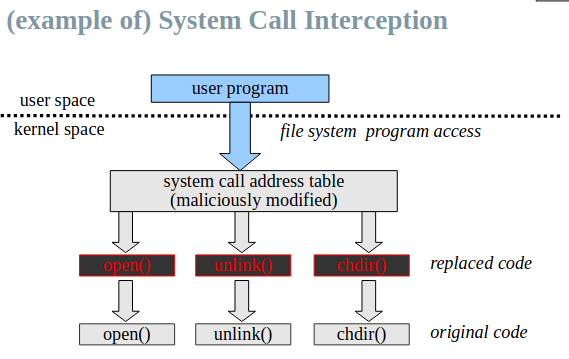
\includegraphics[width=0.6\textwidth]{img/scall interception.png}
  \caption{System call interception}
\end{figure}
In modular operating systems we have a modular structure, which allows
for kernel modules to be loaded.
